\subsection{Animatie met timers}

Een animatie wordt smooth bevonden als er geen frame ontbreekt tijdens het afspelen. Hoe meer frames er per seconde afgebeeld kunnen worden, hoe smoother de animatie oogt. Het gemiddelde consumer-device heeft een refresh rate van 60Hz wat overeenstemt met 60 frames per seconde (fps). Om een animatie zo smooth mogelijk te laten afspelen, wordt er dus over het algemeen gemikt naar een afspeelsnelheid van 60fps.

Om elke seconde 60 frames af te beelden moeten de frames volgens een correct getimed interval de volgende frame afbeelden. In javascript zijn hier twee build-in functies voor beschikbaar, \texttt{setTimeout()} en \texttt{setInterval()}. Op deze manier kan er met een timer om de 16.7ms een nieuwe frame afgebeeld worden om de 60fps playback snelheid te behalen.

\subsection{Problemen met timers}
Bij het gebruik maken van timers wordt er verondersteld van een playback van 60fps omdat de meeste schermen dit hanteren, maar als er een trager scherm gebruikt wordt om deze animatie af te beelden zullen er overtollige frames ingeladen worden niet gerenderd zullen worden door de browser. Een laadtijd van 16.7ms of minder voor elke frame is ook niet gegarandeerd en wordt verder besproken in \textbf{TODO: verwijzing naar performance}. 

\paragraph{Drift in timers}Deze timers zouden er voor zorgen dat er elke gerenderde frame door de brower, de juiste frame van de animatie bevat. Dit kan niet aangenomen worden aangezien er altijd een kleine fout zal bestaan op de wachttijd tot de executie van de opgeroepen functie van de timer. Bij het uitvoeren van onderstaande code die gebasseerd is op een test van \textbf{https://github.com/nodejs/node/issues/21822} blijkt dat veel populaire browsers de kleine fout niet compenseren waardoor de globale timing van de animatie volledig zijn synchronisatie verliest.

\textbf{MAYBE MEER BROWSERS?}

\begin{figure}[H]
\centering
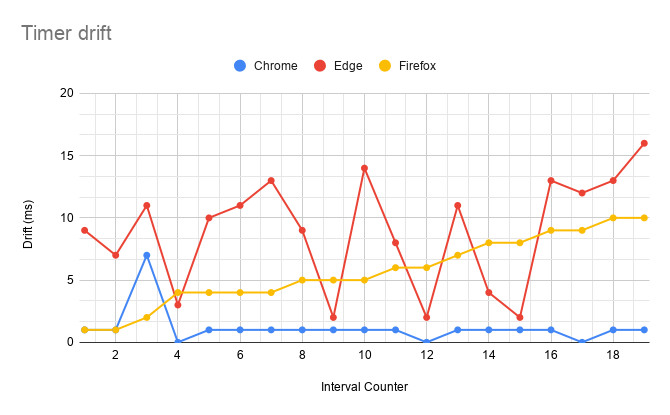
\includegraphics[width=0.8\textwidth]{img/Timer drift.png}
\caption{Timer drift over verschillende populaire browsers} \label{drift}
\end{figure}

\paragraph{Single threaded}
Javascript wordt single-threaded in de browser uitgevoerd. Door deze limitatie kan een taak die getimed staat over x aantal miliseconden pas uitgevoerd worden op de main thread als de event loop op dat moment beschikbaar is om die functie dan uit te voeren. Als er tussen het initialiseren van de timer en het uitvoeren van deze geplande taak een andere taak tussenbeide komt die langere executietijd heeft dan de geplande tijd zal de uitvoering uitgesteld worden tot de event loop terug vrij komt. Ook dit is een deuk in de betrouwbaarheid van timers.

\textbf{hier eventueel een afbeelding}

\subsection{HTTP request frames}

Voor deze test werd gebruik gemaakt van een sprite sheet met 15 frames op (figuur \ref{sheet}) en een animatie snelheid van 30 fps.

\begin{figure}[H]
\centering
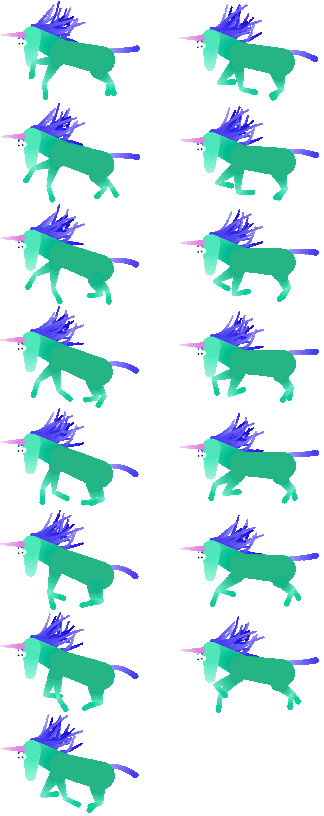
\includegraphics[scale=0.7]{img/charging.png}
\caption{Sprite sheet met 15 frames} \label{sheet}
\end{figure}

Bij de eerste test werdt de hele sprite sheet per frame ingeladen. Dit is om het effect te creeren dat de server elke frame genereerd en doorstuurt naar de client. Dit bleek zeer inefficient te zijn doordat de tijd om de frame op te halen met ethernet rond de 140 ms en met draadloos internet rond de 250 ms ligt (figuur \ref{draadloos} en figuur \ref{ethernet}).

\begin{figure}[H]
	\centering
	\begin{subfigure}[b]{0.45\textwidth}
		\centering
		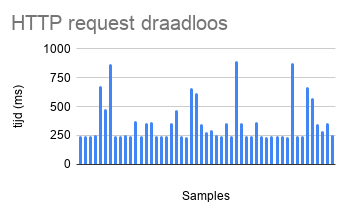
\includegraphics[width=\textwidth]{img/draadloos.png}
		\caption{HTTP request met draadloze verbinding} \label{draadloos}
	\end{subfigure}
	\begin{subfigure}[b]{0.45\textwidth}
		\centering
		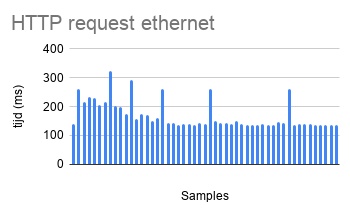
\includegraphics[width=\textwidth]{img/ethernet.png}
		\caption{HTTP request met ethernet verbinding} \label{ethernet}
	\end{subfigure}
\end{figure}

Hoewel de frames asynchroon worden ingeladen (figuur \ref{inladen}) is de animatie alles behalve ideaal. Door lange wachttijden zijn er veel frame skips en door de vele http requests wordt de verbinding gereset om de server niet te overbelasten met 30 requests per seconde (figuur \ref{reset}).

\begin{figure}[H]
\centering
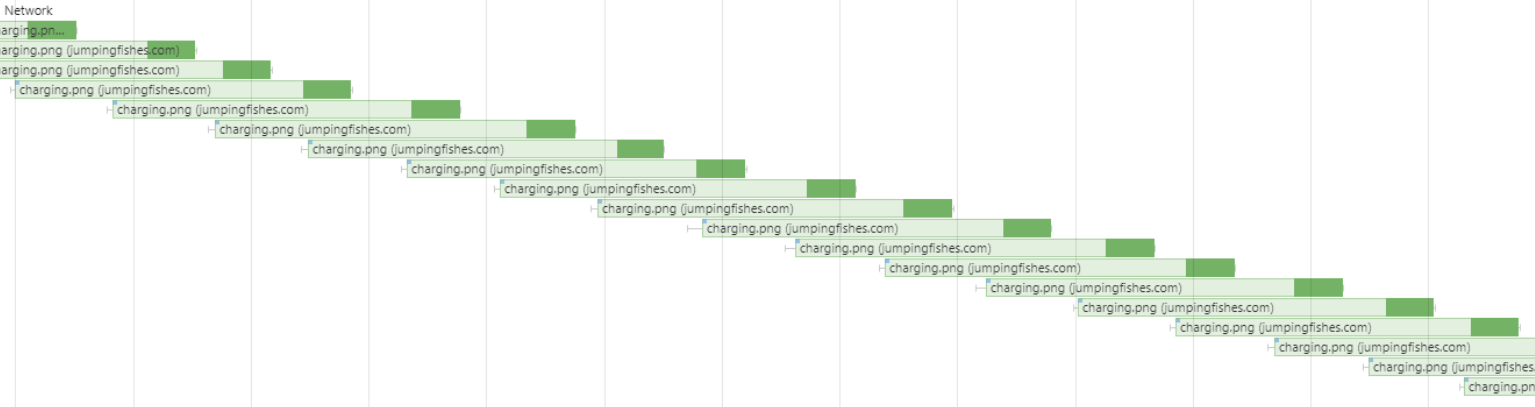
\includegraphics[scale=0.3]{img/inladen.png}
\caption{Inladen van elke frame} \label{inladen}
\end{figure}

\begin{figure}[H]
\centering

\includegraphics[scale=0.7]{img/reset.png}
\caption{Connection reset door teveel requests} \label{reset}
\end{figure}

Bij de tweede test werdt gebruik gemaakt van een buffer. De sprite sheet werdt om de 0.5 seconden ingeladen zodat elke frame tijd had om te displayen ($30 \frac{frames}{sec} \frac{1}{15 frames} = \frac{0.5}{sec} $). Dit creëert het effect dat de server 15 frames genereerd en doorstuurt in 1 keer i.p.v. frame per frame. Dit is duidelijk een verbetering want de server krijgt 15 keer minder requests (figuur \ref{inladen2}) en er zijn geen frame skips meer. Na het inladen van de sheet zal de client de 15 frames achter elkaar drawen zonder te hoeven wachten op de server. Daarna zal de volgende sheet (of buffer) gebruikt worden.

\begin{figure}[H]
\centering
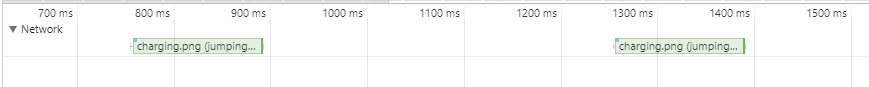
\includegraphics[scale=0.7]{img/inladen2.png}
\caption{Inladen van de buffer} \label{inladen2}
\end{figure}




